\section{Block Sparse K-SVD algorithm applied to BSS}
Last section proves the strength of sparsity based methods applied to blind source separation problem. Inspired by using adaptively learned local dictionary in MMCA/GMCA, we aim to create a new adaptive dictionary learning algorithm combined with BSS. The idea driven behind is simple that, certainly will we acquire a better separation result if we improve the level of sparsity of the dictionary,.\\

A variety of sparse dictionary learnging algorithm have been proposed in the literature for this purpose, based on the K-SVD algorithm. The block-sparse dictionary learning algorithm is proposed by Lihi in \cite{dictionary_block_sparse}. It exploits the hidden structure that is intrinsic in the signals for producing more efficient sparse representations. In the following content, we introduce the theory of this algorithm and try to embed it in the BSS process. \\

\subsection{Problem definition}
Given a set of signals $\mathbf{Y} = \{y_i\} \in R^N$, we wish to find an overcomplete dictionary $\mathbf{\Phi} \ in R^{N\time K}$ whose atoms are sorted in blocks, correspondly the non-zero coefficients representations $\mathbf{X} = \{x_i\}$ are concentrated in a fixed number of blocks. More specifically, suppose dictionary atoms sorted in blocks that enable \textbf{block-sparse} representations of input signals. Each block has its own label, indexed as $d_i$. We claim that a vector $\mathbf{X}\in R^K$ is $k$-block-sparse over $d$ if its non-zero entries are concentrated in $k$ blocks only. This is denoted by 
\begin{equation}
    ||x||_{0,d} = k
\end{equation}
which means there are $k$ number of non-zero blocks having block structure $d$. Figure \ref{block_dict_compare} presents two equivalent examples, The dictionary can be expressed as 5 blocks but with 2-block-sparse presentations.\\

\begin{figure}[!htbp]
\centering
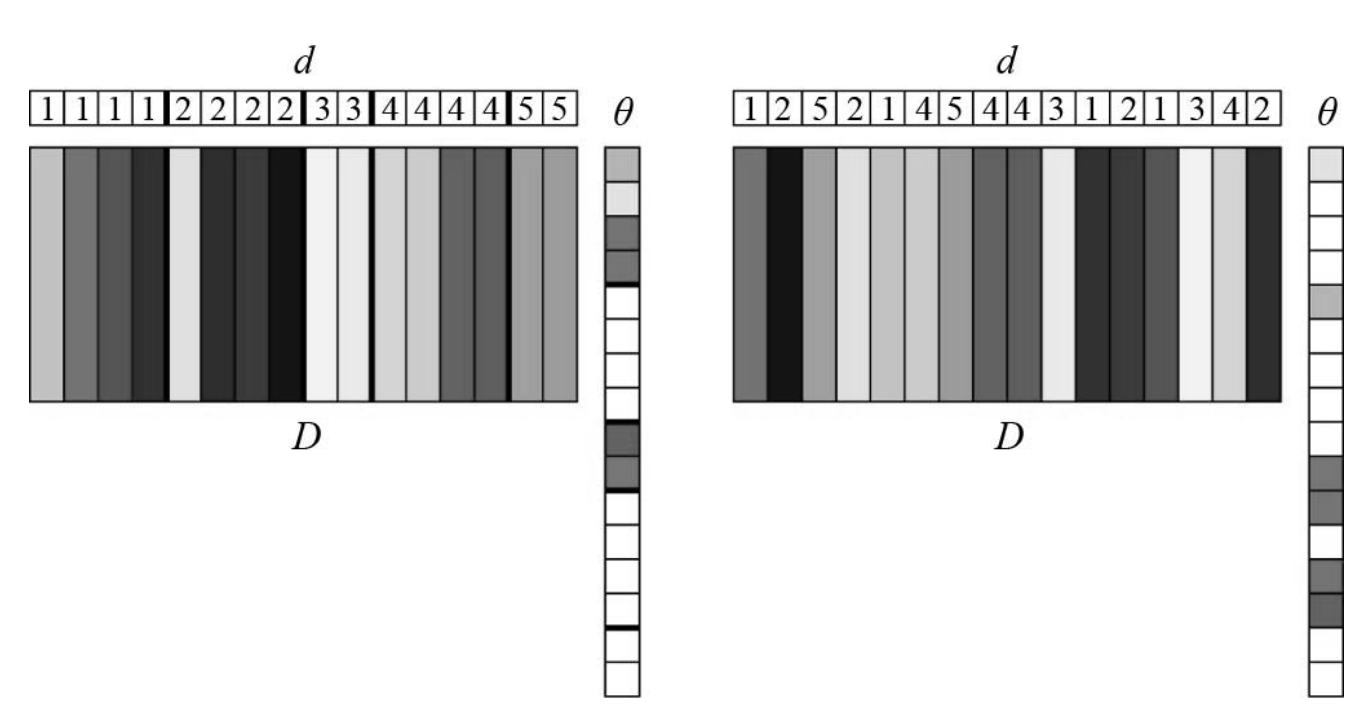
\includegraphics[width=0.7\textwidth]{images/block_dict_compare.png}
\caption{Two equivalent representations with different block structure.}
\label{block_dict_compare}
\end{figure}

We can now formulate the problem is a mathematical way that we intent to find a dictionary $\mathbf{\Phi}$ and a block structure d, with maximal block size s, that lead to optimal k-block sparse representations $\mathbf{X} = \{x_i\}^L_i=1 $ for signals in $\mathbf{Y}$. The objective function is given as below.\\
\begin{equation}
\begin{aligned} 
    \min_{D,d,\mathbf{X}} ||\mathbf{Y} -\mathbf{\Phi}\mathbf{X}||\\
    \text{s.t.} \quad ||x_i||_{0,d} \leq k, \; i = 1,...L\\
    |d_j| \leq s, \; j = 1,....B
    \label{bskvsd_1}
\end{aligned}
\end{equation}

where $d_j$ is the set of indices belonging to block $j$, $s$ is the maximum block size and $B$ is
is the total number of blocks (number of dictionary columns divided by the block size). When the maximal block size is set to 1, the proposed algorithm reduces to normal K-SVD.\\


\subsection{Algorithm Preview}
Like other optimisation problems in previous sections, the problem in Equation \ref{bskvsd_1} is a nonconvex. We therefore adopt the coordinate relaxation technique. The initail dictionary can be set up as a DCT dictionary or any random collection of $K$ signals. Then the block structure is solved by the \textit{sparse aggolmerative clustering} (SAC) algorithm\cite{Johnson1967}. Agglomerative clustering is a `bottom-up' approach who groups according to distance metric (e.g. $\ell_0$ norm).\\

SAC algorithm solves for an optimal block structure refer to input command ($k$ and $s$) while keeping the dictionary fixed.

\begin{equation}
\begin{aligned}
    \left[d^{(m)}, \;\mathbf{\Phi}^{(m)}\right] = \text{arg} \; \min_{X,d} \quad || \mathbf{Y} - \mathbf{\Phi}^{(m-1)}\mathbf{X}||_2 \\
    \text{s.t.} \quad ||x_i||_0,d \leq k, \quad i = 1,...,L\\
    |d_j| \leq s, \; j = 1,....B
\end{aligned}
\end{equation}

After having successfully recovered the optimal block structure. We then solve for new dictionary while keeping $d^{m}$ fixed. The objective function becomes.
\begin{equation}
\begin{aligned}
    \left[\mathbf{X}^{(m)}, \;\mathbf{\Phi}^{(m)}\right] = \text{arg} \; \min_{\Phi,X} \quad || \mathbf{Y} - \mathbf{\Phi}^{(m-1)}\mathbf{X}||_2 \\
    \text{s.t.} \quad ||x_i||_0,d \leq k, \quad i = 1,...,L
\end{aligned}
\label{BKSVD1}
\end{equation}
The author in \cite{dictionary_block_sparse} proposed \textit{block K-SVD} (BK-SVD), a natural extension of the K-SVD algorithm to solve (\ref{BKSVD1}). BK-SVD algorithm employs a similar columnwise atom updating manner as in K-SVD but forces the learned dictionary to have higher sparsity level.\\

We first fix $\mathbf{\Phi}^{m-1}$ and can use any pursuit method (e.g. OMP) to solve (\ref{BKSVD1}) which reduces to.

\begin{equation}
\begin{aligned}
    \mathbf{X}^{(m)} = \text{arg} \; \min_X \quad || \mathbf{Y} - \mathbf{\Phi}\mathbf{X}^{(m-1)}||_2 \\
    \text{s.t.} \quad ||x_i||_0,d \leq k, \quad i = 1,...,L
\end{aligned}
\end{equation}

Then, to obtain $\mathbf{\Phi}^{(m)}$, fix $\mathbf{X}^{(m)}$, $d$ and $\mathbf{Y}$. The calculation procedure is same as K-SVD, where the blocks in the dictionary is updated sequentially, alongside with the corresponding nonzero coefficients in $\mathbf{X}^{(m)}$.\\

The complexity of BKSVD requires $b_s$ times less number of SVD computations than the KSVD algorithm. Their for the convergence rate of BKSVD is significantly faster than KSVD. As proved in \cite{OMP_KSVD}, K-SVD algorithm has a complexity of $O((k)^2K + 2NK)$. Because of the block nature of BK-SVD, we expect BK-SVD to have a complexity of $O((k)^2K + 2NK)$, where $k$ is the sparsity level (number of sparse blocks) and $s$ is the maximal block size.\\

We have now introduced the whole block sparse dictionary learning algorithm. The overall framework of SAC+BK-SVD is summarised below,
\begin{algorithm}[!htbp] 
\caption{Block-sparse Dictionary Update}
\label{alg:Framwork} 
\begin{algorithmic}
\REQUIRE ~~\\%Input
The input signal $\mathbf{Y}$, block sparsity level $k$, and maximal block size $s$.\\
\ENSURE ~~\\ %Output
Learned Dictionary $\mathbf{\Phi}$ with optimal block struture $d$.\\
--------------------------------------------------------\\
\STATE 1. Initialise the dictionary $D(0)$ as the outcome of K-SVD.\\
\STATE 2. For $N$ number of iterations.\\
\STATE \quad - Fix dictionary $\mathbf{\Phi}^{(m-1)}$ and update coefficients $x^{m}$ and block structure $d^{(m)}$ by applying sparse agglomerative clustering.\\
\STATE \quad - Fix the block structure $d^(m)$ and update the dictionary atoms $\mathbf{\Phi}^{(m)}$ by applying BS-SVD.\\
\end{algorithmic}
\end{algorithm}

\subsection{Complexity Analysis}
The standard algorithm for hierarchical agglomerative clustering has a time complexity of ${\displaystyle {\mathcal {O}}(K^{3})}$ (K is the number of dictionary atoms in this occasion). which makes it too slow for even medium data sets.
\clearpage